\documentclass[11pt]{article}
\usepackage[margin=1in]{geometry}
\usepackage[T1]{fontenc}
\usepackage{lmodern}
\usepackage{microtype}
\usepackage{booktabs}
\usepackage{tabularx}
\usepackage{makecell}
\usepackage{graphicx}
\usepackage{enumitem}
\usepackage{caption}
\captionsetup{font=small,labelfont=bf}
\setlist{itemsep=2pt,topsep=4pt}

\title{\textbf{LastSeen: Detector Comparison}}
\author{CIS 5810 Final Project, Group 27\\Rita Wang \quad Isabella Huang \quad Cindy Liang}
\date{November 2026}

\begin{document}
\maketitle

\section{Models compared}
Our baseline (YOLO11s) only knows the 80 COCO classes, so it cannot find many commonly lost items
such as keys, glasses or earbuds. We compared detectors along two axes: \textbf{architecture}
(CNN vs.\ Transformer) and \textbf{vocabulary} (fixed COCO classes vs.\ open-vocabulary detection from a
text prompt).

\begin{table}[h]
\centering\small
\caption{Candidate detectors.}
\label{tab:models}
\begin{tabularx}{\linewidth}{@{}l l l X@{}}
\toprule
Model & Type & Vocabulary & Why we included it \\
\midrule
YOLO11s & CNN, one-stage & COCO-80 & Baseline: small and fast \\
Faster R-CNN & CNN, two-stage & COCO-80 & Classic accurate CNN; tests a stronger CNN design \\
RT-DETR-L & Transformer & COCO-80 & Tests the architecture with the vocabulary held fixed \\
YOLO-World-S & CNN + CLIP text & open & Open vocabulary at YOLO speed \\
YOLOE-11S / 11L & CNN + MobileCLIP text & open & Newer open-vocab YOLO; also accepts image prompts \\
OWLv2 & ViT (Transformer) & open & Strongest open-vocab model on rare objects, but slow \\
\bottomrule
\end{tabularx}
\end{table}

We also ran YOLOE-11S at 1280\,px instead of 640\,px to see how much input resolution helps with small
items, as a preview of SAHI tiling.

\section{Evaluation}
\begin{itemize}
\item \textbf{Data:} 9 desk/room photos and 16 query items, 8 inside COCO (phone, laptop, mouse, cup,
  bottle, book, plant, bowl) and 8 outside (glasses, headphones, pen, keys, earbuds case, wristwatch,
  camera, face mask). We labeled by hand which items appear in each photo.
\item \textbf{Scoring:} a detection counts only if its box overlaps a hand-checked correct box
  (IoU\,$\ge$\,0.5). For each image and item, the best correct box is a hit and the best wrong box is a
  false positive. AP is threshold-free. Recall and precision use each model's default threshold
  (0.25; 0.5 for Faster R-CNN; 0.1 for OWLv2). Runtime is measured on a Colab CPU.
\end{itemize}

\clearpage
\section{Results}
\begin{table}[h]
\centering\small
\setlength{\tabcolsep}{4pt}
\caption{Main results on the shared 9-image benchmark (best per column in bold).}
\label{tab:main}
\begin{tabular}{@{}l ccc cc c c r@{}}
\toprule
 & \multicolumn{3}{c}{mAP} & \multicolumn{2}{c}{Recall} & & Items & CPU \\
\cmidrule(lr){2-4}\cmidrule(lr){5-6}
Model & all & COCO & non-COCO & COCO & non-COCO & Precision & found & ms/img \\
\midrule
YOLO11s (baseline) & 0.42 & 0.84 & 0.00 & 0.79 & 0.00 & 0.79 & 8 & 427 \\
Faster R-CNN & 0.45 & 0.91 & 0.00 & 0.79 & 0.00 & 0.73 & 8 & 11334 \\
RT-DETR-L & 0.47 & \textbf{0.94} & 0.00 & 0.91 & 0.00 & 0.72 & 8 & 1560 \\
\addlinespace
YOLO-World-S & 0.59 & 0.88 & 0.31 & 0.71 & 0.44 & 0.74 & 12 & \textbf{425} \\
YOLOE-11S & 0.53 & 0.78 & 0.29 & 0.71 & 0.25 & 0.68 & 9 & 480 \\
YOLOE-11S @1280 & 0.57 & 0.83 & 0.30 & 0.76 & 0.38 & 0.62 & 11 & 1743 \\
YOLOE-11L & 0.67 & 0.91 & 0.43 & 0.76 & 0.31 & \textbf{0.82} & 10 & 1510 \\
OWLv2 & \textbf{0.79} & 0.93 & \textbf{0.64} & \textbf{1.00} & \textbf{0.88} & 0.43 & \textbf{14} & 22185 \\
\bottomrule
\end{tabular}
\end{table}

\begin{table}[h]
\centering\small
\setlength{\tabcolsep}{3.5pt}
\caption{Per-item AP. Pos.\ = number of images containing the item. Best per row in bold.}
\label{tab:peritem}
\begin{tabular}{@{}l c cccccccc@{}}
\toprule
Item & Pos. & YOLO11s & \makecell{Faster\\R-CNN} & \makecell{RT-\\DETR} & \makecell{YOLO-\\World} & \makecell{YOLOE\\-S} & \makecell{YOLOE-S\\@1280} & \makecell{YOLOE\\-L} & OWLv2 \\
\midrule
\multicolumn{10}{@{}l}{\textit{Inside COCO}} \\
\quad cell phone & 6 & 0.50 & 0.74 & 0.71 & 0.58 & 0.54 & 0.48 & 0.81 & \textbf{0.86} \\
\quad laptop & 6 & 0.93 & 0.98 & \textbf{1.00} & 0.90 & 0.81 & 0.81 & 0.93 & \textbf{1.00} \\
\quad mouse & 4 & 0.67 & \textbf{0.95} & 0.88 & 0.69 & 0.42 & 0.42 & 0.62 & \textbf{0.95} \\
\quad cup & 6 & \textbf{1.00} & 0.92 & \textbf{1.00} & 0.94 & 0.90 & \textbf{1.00} & \textbf{1.00} & \textbf{1.00} \\
\quad bottle & 2 & \textbf{1.00} & \textbf{1.00} & \textbf{1.00} & \textbf{1.00} & \textbf{1.00} & \textbf{1.00} & \textbf{1.00} & \textbf{1.00} \\
\quad book & 5 & 0.79 & 0.93 & 0.90 & 0.94 & 0.59 & \textbf{0.97} & 0.93 & 0.66 \\
\quad potted plant & 3 & 0.87 & 0.76 & \textbf{1.00} & \textbf{1.00} & \textbf{1.00} & \textbf{1.00} & \textbf{1.00} & \textbf{1.00} \\
\quad bowl & 2 & \textbf{1.00} & \textbf{1.00} & \textbf{1.00} & \textbf{1.00} & \textbf{1.00} & \textbf{1.00} & \textbf{1.00} & \textbf{1.00} \\
\midrule
\multicolumn{10}{@{}l}{\textit{Outside COCO}} \\
\quad glasses & 2 & 0.00 & 0.00 & 0.00 & 0.50 & 0.00 & 0.50 & 0.50 & \textbf{1.00} \\
\quad headphones & 2 & 0.00 & 0.00 & 0.00 & 0.50 & 0.50 & 0.50 & 0.50 & \textbf{1.00} \\
\quad pen & 6 & 0.00 & 0.00 & 0.00 & 0.46 & 0.38 & 0.54 & 0.91 & \textbf{0.93} \\
\quad keys & 1 & 0.00 & 0.00 & 0.00 & 0.00 & 0.00 & 0.00 & 0.00 & 0.00 \\
\quad earbuds case & 2 & 0.00 & 0.00 & 0.00 & 0.00 & 0.42 & \textbf{0.83} & 0.50 & 0.70 \\
\quad wristwatch & 1 & 0.00 & 0.00 & 0.00 & 0.00 & 0.00 & 0.00 & 0.00 & \textbf{0.50} \\
\quad camera & 1 & 0.00 & 0.00 & 0.00 & \textbf{1.00} & \textbf{1.00} & 0.00 & \textbf{1.00} & \textbf{1.00} \\
\quad face mask & 1 & 0.00 & 0.00 & 0.00 & 0.00 & 0.00 & 0.00 & 0.00 & 0.00 \\
\bottomrule
\end{tabular}
\end{table}



\clearpage
\begin{figure}[t]
\centering
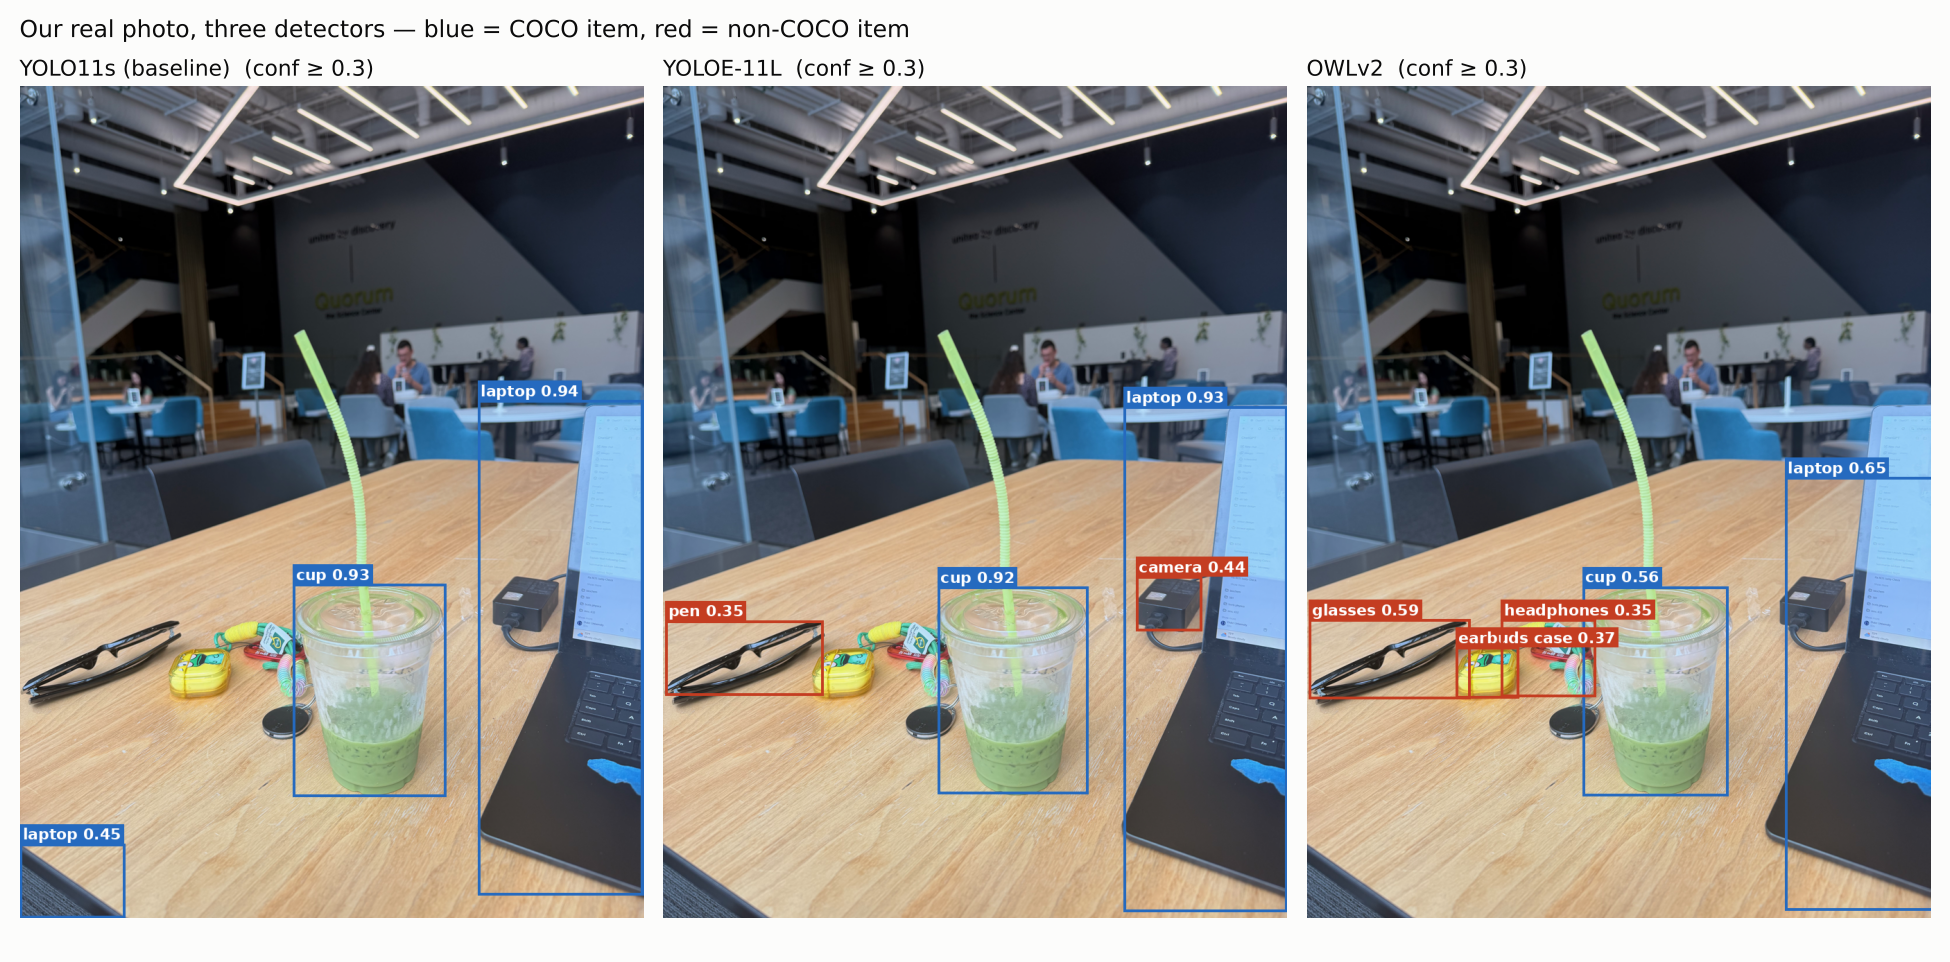
\includegraphics[width=\linewidth]{example_9jpg.png}
\caption{Our real photo, three detectors (boxes with confidence $\ge$ 0.3; blue = COCO item, red = non-COCO
item). The baseline only labels COCO items (plus a false ``laptop'' in the corner). YOLOE-11L mislabels the
sunglasses as ``pen'' and the charger as ``camera''. OWLv2 correctly finds the sunglasses and the earbuds case,
but also puts a wrong ``headphones'' box on the keychain. No model finds the keys.}
\label{fig:example}
\end{figure}

\paragraph{Key findings.}
\begin{itemize}
\item \textbf{The vocabulary matters more than the architecture.} All three closed-set models (one-stage
  CNN, two-stage CNN, Transformer) score 0 on every non-COCO item.
\item \textbf{On COCO items, stronger architectures help.} RT-DETR (0.94), OWLv2 and Faster R-CNN all
  beat the baseline (0.84), but Faster R-CNN is about 25$\times$ slower than the baseline.
\item \textbf{Open-vocabulary models find the missing items.} OWLv2 is the most accurate overall
  (mAP 0.79, 14 of 16 item types found). It is the only model that found the sunglasses in our real
  photo (Figure~\ref{fig:example}) and the wristwatch, but it takes about 22\,s per image on CPU (about 50$\times$ the baseline).
  YOLOE-11L (mAP 0.67) and YOLO-World (0.59, at baseline speed) offer a much better speed/accuracy
  trade-off.
\item \textbf{Resolution helps small items.} YOLOE-11S at 1280\,px raises non-COCO recall from 0.25 to
  0.38, which supports adding SAHI tiling.
\item \textbf{Keys and face masks are still missed by every model.} OWLv2 also has low precision
  (0.43): it finds more items but produces more wrong boxes.
\end{itemize}

\paragraph{Limitations and next steps.}
The benchmark is small (1--6 positive images per item), so we read trends rather than small differences.
Next we will collect 30--50 of our own photos with box labels (low light, blur, clutter), add SAHI
tiling, and report the same tables every iteration.

\end{document}
